\documentclass[12pt,a4paper]{article}
% \usepackage[utf8]{inputenc} % fontspecと併用時は不要
\usepackage[japanese]{babel}
\usepackage{amsmath}
\usepackage{amsfonts}
\usepackage{amssymb}
\usepackage{geometry}
\usepackage{graphicx}
\usepackage{enumitem}
\usepackage{fancyhdr}
\usepackage{verbatim}
\usepackage{tcolorbox}
\tcbuselibrary{breakable}

% 日本語改行設定
\usepackage{xeCJK}
\usepackage{indentfirst}
\setlength{\parindent}{1em}

% 日本語フォント設定
\usepackage{fontspec}
\setmainfont{Hiragino Mincho Pro}
\setsansfont{Hiragino Sans}
\setmonofont{Menlo}
\setCJKmainfont{Hiragino Mincho Pro}
\setCJKsansfont{Hiragino Sans}
\setCJKmonofont{Menlo}
% ページ設定
\geometry{margin=1.5cm}
\pagestyle{fancy}
\fancyhf{}
\fancyhead[L]{プログラミング応用 第四回}
\fancyhead[R]{演習問題解説}
\fancyfoot[R]{\ifnum\value{page}=1\small（裏面に続く）\fi}
\fancyfoot[C]{\thepage}
\renewcommand{\headrulewidth}{0.4pt}
\renewcommand{\footrulewidth}{0.4pt}

% 問題番号のカウンター
\newcounter{problem}
\setcounter{problem}{0}

% シンプルな問題環境
\newenvironment{problem}[1][]{
    \refstepcounter{problem}
    \vspace{1em}
    \noindent
    \textbf{問\arabic{problem}} #1
    %\vspace{0.5em}
    %\par
}{
    \vspace{1em}
}

% 解答環境
\newenvironment{solution}{
    \vspace{0.5em}
    \begin{tcolorbox}[colback=white, colframe=black, boxrule=1pt, arc=0mm, breakable]
    \noindent
    \textbf{【解答】}
    \vspace{0.3em}
}{
    \end{tcolorbox}
    \vspace{1em}
}

\begin{document}

% ヘッダー情報
\begin{center}
    {\Large \textbf{プログラミング応用 第四回}}\\[0.5em]
    {\large \textbf{演習問題解説}}\\[1em]
\end{center}


\begin{problem}
次の問いに答えよ.
\begin{enumerate}
\item 次の図\ref{fig:graph_ex}で表されるグラフの隣接行列 $A$ を書け (\textbf{1点}).

\begin{figure}[h]
    \begin{center}
    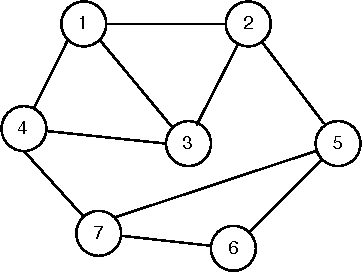
\includegraphics[width=0.45\textwidth]{graph_ex.drawio.pdf}
    \caption{グラフ \label{fig:graph_ex}}
    \end{center}
\end{figure}

\item グラフ $G=(V,E)$ の三角形の個数を $\mathrm{Tri}(G)$ とする. ここで三角形とは, 相異なる三つの頂点からなる集合 $\{u,v,w\}\subseteq V$ であって, $\{u,v\},\{v,w\},\{w,u\}\in E$ を満たすものを表す. 例えば上の図で表されるグラフの三角形は$\{1,2,3\},\{1,3,4\},\{5,6,7\}$の3つである. このとき, \[\mathrm{Tri}(G) = \frac{1}{6}\mathrm{tr}(A^3)\]を示せ. ここで$\mathrm{tr}(M)$は行列$M$のトレース (対角成分の和) を表す (\textbf{1点}).

\end{enumerate}

\end{problem}

\begin{solution}

\paragraph*{1の解説.}
隣接行列$A$は
\begin{align*}
  A = \begin{pmatrix}
    0 & 1 & 1 & 1 & 0 & 0 & 0 \\
    1 & 0 & 1 & 0 & 1 & 0 & 0 \\
    1 & 1 & 0 & 1 & 0 & 0 & 0 \\
    1 & 0 & 1 & 0 & 0 & 0 & 1 \\
    0 & 1 & 0 & 0 & 0 & 1 & 1 \\
    0 & 0 & 0 & 0 & 1 & 0 & 1 \\
    0 & 0 & 0 & 1 & 1 & 1 & 0 
  \end{pmatrix}
\end{align*}

\paragraph*{2の解説.}
グラフ$G=(V,E)$の任意の三角形$\{u,v,w\}$に対して$3!$個の長さ3の閉路が対応する:
\begin{align*}
(u,v,w,u), (u,w,v,u), (v,u,w,v), (v,w,u,v), (w,u,v,w), (w,v,u,w).
\end{align*}
従って, 長さ3の閉路の個数を$N$とすると, $N = \mathrm{Tri}(G) \times 6$が成り立つ. 問2(1)より, $N=\mathrm{tr}(A^3)$なので, $\mathrm{Tri}(G) = \frac{1}{6}\mathrm{tr}(A^3)$が得られる.

\end{solution}

\newpage

\begin{problem}
    以下の各小問に答えよ.
    \begin{enumerate}
    \item グラフ $G=(V,E)$ の隣接行列を$A$とする. 任意の $\ell\ge 0$ と $u,v\in V$ に対して, $A^\ell_{u,v}$ は $u$ から $v$ への長さ $\ell$ の路の本数に等しいことを示せ (\textbf{1点}).
    \item $n$頂点のグラフ $G=(V,E)$ に対して, $G$が四角形を\textbf{含むかどうか}を $O(n^3)$時間で判定するアルゴリズムを記述せよ. ここで四角形とは, 相異なる四つの頂点からなる集合 $\{a,b,c,d\}\subseteq V$ であって, $\{a,b\},\{b,c\},\{c,d\},\{d,a\}\in E$ を満たすものを表す. 例えば図\ref{fig:graph_ex}で表されるグラフは四角形$\{1,2,3,4\}$を含む. しかし, このグラフから辺$\{2,3\}$を取り除いて得られるグラフは四角形を含まない (\textbf{1点}).
    \item 小問2と同じ問題を $O(n^2)$時間で判定するアルゴリズムを記述せよ. 記述したアルゴリズムが実際に $O(n^2)$時間で動作すること, およびそれが正しく判定することも簡単に説明せよ (\textbf{2点}).
    \end{enumerate}
\end{problem}

\begin{solution}
\paragraph*{1の証明.}
  二頂点$u,v\in V$および$\ell\ge 0$に対して, 長さ$\ell$の$uv$路の集合を$P^{\ell}_{u,v}$とする. すなわち, $A^\ell_{u,v}=|P^{\ell}_{u,v}|$を示せばよい. これを$\ell$に関する帰納法で示す.
  $\ell=0$のとき, $P^0_{u,u}=\{(u)\}$, $P^0_{u,v}=\emptyset$ ($u\ne v$) であるから, $A^0_{u,v}=|P^0_{u,v}|$が成り立つ. 以降は$\ell\ge 1$の場合を考える.
  任意のパス$(u_0,\dots,u_{\ell})\in P^{\ell}_{u,v}$は二つのパス $(u_0,\dots,u_{\ell-1})$と$(u_{\ell-1},u_{\ell})$の結合として表せる.
  特に, $u_{\ell-1}$は$u_{\ell}=v$の隣接頂点である. 従って
  \begin{align*}
    P^{\ell}_{u,v} = \bigcup_{\substack{w\colon \text{$u$の隣接頂点} \\ (u_0,\dots,u_{\ell-1})\in P^{\ell-1}_{u,w}}} \{ (u_0,\dots,w,v) \}.
  \end{align*}
  特に, $|P^{\ell}_{u,v}| = \sum_{w\colon \text{$u$の隣接頂点}} |P^{\ell-1}_{u,w}| = \sum_{w\colon \text{$u$の隣接頂点}} A^{\ell-1}_{u,w}$が成り立つ (ここで$\ell-1$に対する帰納法の仮定を用いた).
  従って, $|P^\ell_{u,v}|=A^\ell_{u,v}$が成り立つ.

\paragraph*{2の解説.} 与えられたグラフの隣接行列を$A$とする. $O(n^3)$時間で$A^2$を計算し, $A^2_{u,v}\ge 2$を満たす$u\ne v$が存在するかどうかを確認すればよい.

\paragraph*{3の解説.} 与えられたグラフを$G=(V,E)$とする. 頂点$u$の隣接頂点の集合を$N(u)$とする. 以下のアルゴリズムを考える:

\begin{enumerate}
  \item 二次元$n\times n$リスト $C$を用意し, 全ての成分を$0$で初期化する.
  \item 全ての$u\in V$に対して以下を実行する:
  \begin{enumerate}
    \item 全ての$v,w\in N(u)$ (ただし$v\ne w$)に対して, $C_{v,w}\leftarrow C_{v,w}+1$とする.
    \item $C_{v,w}\ge 2$ならば, 「Yes」を出力して終了.
  \end{enumerate}
  \item 最後まで終了しなければ, 「No」を出力して終了.
\end{enumerate} このアルゴリズムは$O(n^2)$時間で動作する. 実際, もしも2の反復が$n^2+1$回実行されてもなお終了していないとき, $C$の成分の個数は$n^2$個なので, 必ずどこかの成分は$2$回以上$+1$されているはずであるが, その瞬間にアルゴリズムは終了するため, 矛盾する.
\end{solution}
\begin{problem}
二つの実数 $a,b\in\mathbb{R}$ に対して, $a\oplus b = \min\{a,b\}$, $a\otimes b = a+b$ と定義する. 例えば, $1\oplus 2 = 1$, $1\otimes 2 = 3$ である.
二つの行列$A,B\in\mathbb{R}^{n\times n}$ に対して, $(\oplus,\otimes)$ をそれぞれ加算と乗算として用いて定義される行列積
\begin{align*}
    (A \circledast B)_{i,j} &= (A_{i,1} \otimes B_{1,j}) \oplus \cdots \oplus (A_{i,n} \otimes B_{n,j}) \\
    &= \bigoplus_{k=1}^n (A_{i,k} \otimes B_{k,j})
\end{align*}
を定め, $A^{\circledast k}$ を, $k=1$のときは $A$ とし, $k>1$のときは $A^{\circledast (k-1)} \circledast A$ と定義する. 以下の問いに答えよ.

\begin{enumerate}
    \item 以下の行列$A,B$に対して, $A\circledast B$ を計算せよ (\textbf{1点}).
    \begin{align*}
        A = \begin{pmatrix}
            1 & 2 \\
            3 & 4
        \end{pmatrix}, \quad
        B = \begin{pmatrix}
            5 & 6 \\
            7 & 8
        \end{pmatrix}
    \end{align*}

    \item 図\ref{fig:graph_ex}で表されるグラフ $G$ に対し, 行列 $B$ を (\textbf{1点}).
    \begin{align*}
        B_{u,v} = \begin{cases}
            1 & \text{if }\{u,v\}\in E, \\
            \infty & \text{otherwise}.
        \end{cases}
    \end{align*}    
    とする (すなわち, 隣接行列の$0$成分を$\infty$に置き換えたものである). このとき, $B^{\circledast 3}$を計算せよ.

    \item $n$頂点の\textcolor{red}{非負}重み付き無向グラフ $G=(V,E,w)$ に対し, 行列 $B\in (\mathbb{R}\cup\{\infty\})^{n\times n}$ を
    \begin{align*}
        B_{u,v} = \begin{cases}
            \textcolor{red}{ 0 }& \textcolor{red}{\text{if }u=v,} \\
            w(u,v) & \text{if }\{u,v\}\in E, \\
            \infty & \text{otherwise}.
        \end{cases}
    \end{align*}
    とする. このとき, $B^{\circledast n}$ は全点対最短経路問題の解であることを示せ. ただし, $G$は連結, すなわち任意の$u,v\in V$に対して$u$から$v$への路が存在することを仮定する (\textbf{2点}).
\end{enumerate}
\end{problem}

\begin{solution}
\paragraph*{1の解説.}
\begin{align*}
  A \circledast B = \begin{pmatrix}
    6 & 7 \\
    8 & 9
  \end{pmatrix}
\end{align*}
\paragraph*{2の解説.}

どの頂点ペアも長さ$3$の路が存在するので, 全ての成分が$3$である行列が正解.

\[
\begin{pmatrix}
3 & 3 & 3 & 3 & 3 & 3 & 3 \\
3 & 3 & 3 & 3 & 3 & 3 & 3 \\
3 & 3 & 3 & 3 & 3 & 3 & 3 \\
3 & 3 & 3 & 3 & 3 & 3 & 3 \\
3 & 3 & 3 & 3 & 3 & 3 & 3 \\
3 & 3 & 3 & 3 & 3 & 3 & 3 \\
3 & 3 & 3 & 3 & 3 & 3 & 3
\end{pmatrix}
\]
対角成分の指定が抜けていたので, これ由来で間違えた回答も丸にしています.

\paragraph*{3の解説.}
\textcolor{red}{辺重みの非負性と$B_{u,v}=0$ ($u=v$) の定義を指定し忘れてました...}
$B^k_{u,v}$は$u$から$v$への長さ$k$以下の路の重みの最小値を表すことを$k$についての帰納法で証明すればよい.

\end{solution}

\begin{problem}
    グラフ $G=(V,E)$ に対してSeidel法を適用する際に考える2-ホップグラフ $\widetilde{G}$ の全点対距離を $(\widetilde{\mathrm{dist}}(u,v))_{u,v\in V}$ とする. このとき, 全ての二頂点$u,v\in V$および$v$に隣接する頂点$i$ に対して, $\widetilde{\mathrm{dist}}(u,i) \le \widetilde{\mathrm{dist}}(u,v)+1$ が成り立つことを示せ (\textbf{1点}).
\end{problem}

\begin{solution}
\paragraph*{解説.}
  $\widetilde{G}$上で$v$と$i$は隣接しているので, $\widetilde{\mathrm{dist}}(u,i) \le \widetilde{\mathrm{dist}}(u,v)+1$ が成り立つ.

\end{solution}

\end{document}
